\documentclass[12pt, letterpaper]{article}

\usepackage[english]{babel} % Sets the language and regional settings for English documents
\usepackage[utf8]{inputenc} % Allows the use of UTF-8 characters in the document
\usepackage[T1]{fontenc} % Specifies the font encoding
\usepackage[margin=2cm]{geometry} % Sets the page margins
\usepackage{makeidx} % Enables the creation of indexes
\usepackage{natbib} % Provides flexible bibliography support
\usepackage{url} % Allows the use of URLs
\usepackage{enumitem} % Customizes the appearance of lists
\usepackage{listings} % Provides syntax highlighting for code listings
\usepackage[dvipsnames]{xcolor} % Allows the use of colors
\usepackage{parskip} % Modifies paragraph spacing
\usepackage{graphicx} % Enables the inclusion of graphics
\usepackage{tikz} % Allows the creation of graphics and diagrams
\usepackage{float}
\usepackage{hyperref} % Enables the creation of hyperlinks
\hypersetup{
    pdfpagemode=UseNone,
    pdfstartview=FitH,
    pdftitle={Previo 2 - Análisis Senoidal Permanente},
    pdfauthor={Ugartechea González Luis Antonio, Tepal Briseño Hansel Yael},
    bookmarksnumbered=false
}
\usepackage{amsmath} % Provides additional math environments and commands
\usepackage{circuitikz} % Allows the creation of electrical circuits
\usepackage{adjustbox} % Adjusts the size of the circuit diagrams
\usepackage{arydshln} % Allows the use of dashed lines in tables

\usetikzlibrary{shapes.geometric, positioning}

\graphicspath{ {./img/} } % Sets the path for the graphics

\newlist{biblio}{enumerate}{1}
\setlist[biblio,1]{label=[\arabic*]}

\makeindex

\begin{document}

\begin{titlepage}

	\begin{tikzpicture}[remember picture,overlay]
		\node[anchor=north west, inner sep=30] at (current page.north west) {
			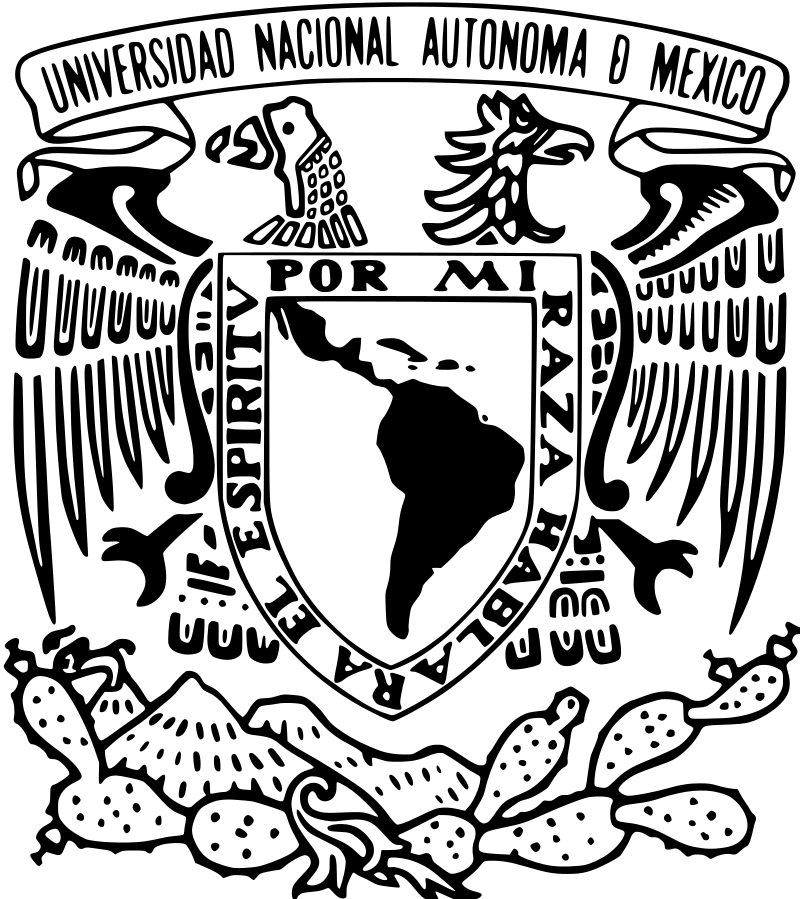
\includegraphics[width=4cm]{escudoUNAM.png}
		};

		\node[anchor=north east, inner sep=30] at (current page.north east) {
			
\includegraphics[width=4cm]{escudoFI.png}
		};
	\end{tikzpicture}

	\begin{center}
		\vspace*{3cm}

		\Huge
		\textbf{Previo 2 - Análsis Senoidal Permanente de Circuitos Lineales}

		\vspace{2.5cm}

		\Huge
		\textbf{Facultad de Ingeniería}\\
		Circuitos Eléctricos\\
		Semestre 2026-1\\

		\vspace{2.5cm}

		\textbf{Grupo:} 4
        \textbf{}

		\vspace{2.5cm}

		\Huge
		Ugartechea González Luis Antonio\\
		Tepal Briseño Hansel Yael \\
		\textbf{Fecha de entrega:} 26/08/2025
		\vspace{2.5cm}
	\end{center}

\end{titlepage}

\section{\texorpdfstring{Determine en función de \(r_g\), \(r_L\), \(R\), \(L\) y \(\omega\) el ángulo de defasamiento entre los voltajes \(V_o\) y \(V_i\) de la figura \ref{fig:figura1}.}{Determine en funcion de rg, rL, R, L y omega el angulo de defasamiento entre los voltajes Vo y Vi de la figura 1.}}

\begin{figure}[H]
    \centering
    \begin{circuitikz}[american, dot/.style={circle, inner sep=1.5pt, fill=black}]
        \draw (0,0) 
            to[V, invert, l={$V_i$}] (0,2)
            to[R, l={$r_g$}, i={$i(t)$}] (0,4)
            to[L, l={$L$}] (3,4)
            to[R, l={$r_L$}] (4.5,4) -- (6,4)
            (0,0) -- (6,0)
            (6,4) to[R, l_={$R$}] (6,0)
        ;
        
        % Add annotations for the detailed equations
        \node[anchor=east] at (-0.5,1) {\footnotesize $V_i = 6 \sin(\omega t)$};
        \node[anchor=south] at (6,0.5) {\footnotesize $R = 200\,\Omega$};

        %Omega
        \node[left] at (-0.2,0.5) {\footnotesize $\omega = 4000 \pi \, \mathrm{rad}/\mathrm{s}$};

        % Terminales de salida
        \draw
            (6,4) -- (7,4) node[dot, label=right:{$+$}] (pvout) {}
            (6,0) -- (7,0) node[dot, label=right:{$-$}] (nvout) {}
        ;

        % Etiqueta de Vout
        \node[right] at (7.2,2) {$V_{o}(s)$};
    \end{circuitikz}
    \caption{Circuito RL}
    \label{fig:figura1}
\end{figure}

\section{Determine en función de \(r_g\), \(R\), \(C\) y \(\omega\) el ángulo de defasamiento entre los voltajes \(V_o\) y \(V_i\) de la figura \ref{fig:figura2}.}

% \begin{figure}[H]
%     \centering
%     \begin{circuitikz}[american, dot/.style={circle, inner sep=1.5pt, fill=black}]
%         \draw (0,0) 
%             to[V, invert, l=\mbox{$V_i = 6 sen (\,\omega)t$}] (0,2)
%             to[R, l=$r_g$, i=$i(t)$] (0,4)
%             to[R, l=\mbox{$R = 500\,\Omega$}] (4.5,4) -- (6,4)
%             (0,0) -- (6,0)
%             l=\mbox{$C = 0.22\,\mu\mathrm{F}$}
%         ;

%         %Omega
%         \draw
%             l=\mbox{$C = 0.22\,\mu\mathrm{F}$}
%         ;

%         % Terminales de salida
%         \draw
%             (6,4) -- (7,4) node[dot, label=right:$+$] (pvout) {}
%             (6,0) -- (7,0) node[dot, label=right:$-$] (nvout) {}
%         ;

%         % Etiqueta de Vout
%         \path
%             let \p1 = (pvout), \p2 = (nvout) in
%             node[right] at ($(\p1)!.5!(\p2)$) {$V_{o}(s)$}
%         ;
%     \end{circuitikz}
%     \caption{Circuito RC}
%     \label{fig:figura2}
% \end{figure}

\section{Determine en función de \(r_g\), \(R_1\), \(r_L\), \(R_2\), \(L\), \(C\) y \(\omega\) el ángulo de defasamiento entre la corriente \(i_e\) y el voltaje \(V_o\) del circuito de la figura \ref{fig:figura3}, con el interruptor \(S\) abierto y cerrado.}

% \begin{figure}[H]
%     \centering
%     \begin{circuitikz}[american, dot/.style={circle, inner sep=1.5pt, fill=black}]
%         \draw (0,0) 
%             to[V, invert, l=\mbox{$V_i = 6 sen (\,\omega)t$}] (0,2)
%             to[R, l=$r_g$, i=$i(t)$] (0,4)
%             to[R, l=\mbox{$R = 500\,\Omega$}] (4.5,4) -- (6,4)
%             (0,0) -- (6,0)
%             l=\mbox{$C = 0.22\,\mu\mathrm{F}$}
%         ;

%         %Omega
%         \draw
%             l=\mbox{$C = 0.22\,\mu\mathrm{F}$}
%         ;

%         % Terminales de salida
%         \draw
%             (6,4) -- (7,4) node[dot, label=right:$+$] (pvout) {}
%             (6,0) -- (7,0) node[dot, label=right:$-$] (nvout) {}
%         ;

%         % Etiqueta de Vout
%         \path
%             let \p1 = (pvout), \p2 = (nvout) in
%             node[right] at ($(\p1)!.5!(\p2)$) {$V_{o}(s)$}
%         ;
%     \end{circuitikz}
%     \caption{Circuito RC}
%     \label{fig:figura3}
% \end{figure}

% \section{Bibliography}

% \begin{biblio}
% 	%for: https://www.poli.edu.co/blog/poliverso/diseno-digital-que-es
% 	\item \textit{Diseño digital: qué es y por qué es importante.} (2021, August 26). Poliverso. Retrieved October 16, 2024, from: \textcolor{blue}{\underline{\url{https://www.poli.edu.co/blog/poliverso/diseno-digital-que-es}}}
% 	%for: https://www.sky6cancun.com/marketing/diseno-grafico/diseno-digital-que-es-y-para-que-sirve/
% 	\item \textit{Diseño digital: qué es y para qué sirve.} (2021, August 26). Sky6Cancún. Retrieved October 16, 2024, from: \textcolor{blue}{\underline{\url{https://www.sky6cancun.com/marketing/diseno-grafico/}}}
% \end{biblio}

\end{document}
